\section{正态总体均值和方差的区间估计}

\subsection{单个正态总体参数的置信区间}

正态总体 $ N\left(\mu, \sigma^{2}\right) $ 是最常见的分布,
下面我们讨论它的两个参数 $ \mu $ 和 $ \sigma^{2} $ 的置信区间.
设 $ X_{1}, X_{2}, \cdots, X_{n} $ 是来自总体 $ X $ 的样本.
\begin{theorem}[$\sigma^{2} $ 已知时 $ \mu $ 的置信区间]
    $\sigma^{2} $ 已知,选择枢轴量 $\displaystyle \frac{\bar{X}-\mu}{\sigma / \sqrt{n}}$,
    得到 $ \mu $ 的置信水平为 $ 1-\alpha $ 的置信区间为 $ \left(\bar{X} \pm z_{\alpha / 2} \sigma / \sqrt{n}\right) .$
\end{theorem}
\begin{theorem}[$\sigma^{2} $ 未知时 $ \mu $ 的置信区间]
    $\sigma^{2} $ 未知,由于枢轴量 $\displaystyle \frac{\bar{X}-\mu}{\sigma / \sqrt{n}} \sim N(0,1) $ 中含有未知参数 $ \sigma $,
    故不能采用. 而 $\displaystyle \frac{\bar{X}-\mu}{S / \sqrt{n}} \sim t(n-1)$ 含有待估计参数 $ \mu $,
    且不含有其他未知参数,则使用 $\displaystyle \frac{\bar{X}-\mu}{S / \sqrt{n}} $ 作为枢轴量 (见图 \ref{tfweidian}(a)), 得
    $$P\left\{-t_{\alpha / 2}(n-1)<\frac{\bar{X}-\mu}{S / \sqrt{n}}<t_{\alpha / 2}(n-1)\right\}=1-\alpha$$
    即
    $$P\left\{\bar{X}-t_{\alpha / 2}(n-1) S / \sqrt{n}<\mu<\bar{X}+t_{\alpha / 2}(n-1) S / \sqrt{n}\right\}=1-\alpha$$
    因此,$\mu $ 的置信水平为 $ 1-\alpha $ 的置信区间为
    $$\left(\bar{X}-t_{\alpha / 2}(n-1) S / \sqrt{n}, \bar{X}+t_{\alpha / 2}(n-1) S / \sqrt{n}\right)$$
    常缩写为 $$\left(\bar{X} \pm t_{a / 2}(n-1) S / \sqrt{n}\right) .$$
\end{theorem}

\begin{figure}[H]
    \centering
    \subfigure[]{
        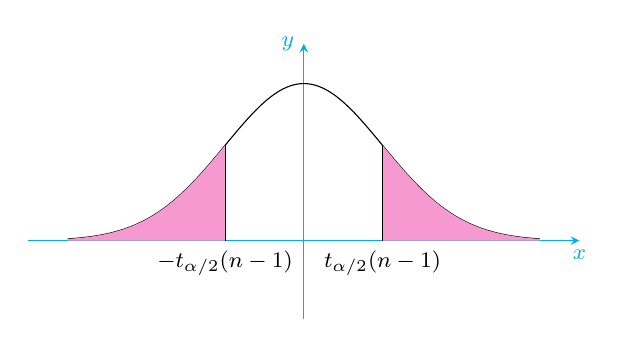
\begin{tikzpicture}[->,samples=100,>=stealth,font=\footnotesize,yscale=5]
            \def\xmin{-3.5}
            \def\xmax{3.5}
            \def\ymin{-.2}
            \def\ymax{.5}
            \def\a{0.398942}
            \draw[->,cyan](\xmin,0)--(0,0)--(\xmax,0)node[below]{$x$};
            \draw[->,cyan](0,\ymin)--(0,\ymax)node[left]{$y$};

            \draw[scale=1,domain=-3:3,smooth,variable=\x,black,-] plot ({\x},{\a*exp(-\x*\x/2)});

            \fill[color=magenta!40] (1,0) -- plot[domain=1:3,smooth,variable=\x] ({\x},{\a*exp(-\x*\x/2)}) -- (3,0) --cycle;
            \node[below] at (1,0) {$t_{\alpha/2}(n-1)$};
            \draw[-] (1,0)--plot[domain=1:1,smooth,variable=\x] ({\x},{\a*exp(-\x*\x/2)});

            \fill[color=magenta!40] (-1,0) -- plot[domain=-1:-3,smooth,variable=\x] ({\x},{\a*exp(-\x*\x/2)}) -- (-3,0) --cycle;
            \node[below] at (-1,0) {$-t_{\alpha/2}(n-1)$};
            \draw[-] (-1,0)--plot[domain=-1:-1,smooth,variable=\x] ({\x},{\a*exp(-\x*\x/2)});
        \end{tikzpicture}
    }
    \subfigure[]{
        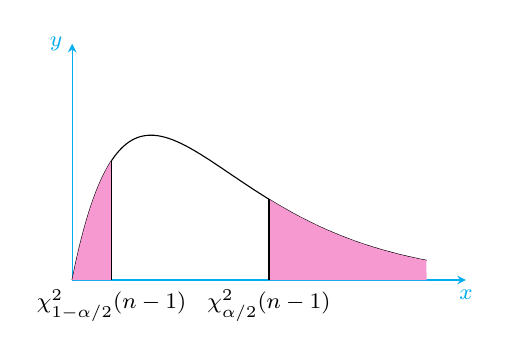
\begin{tikzpicture}[->,samples=100,>=stealth,font=\footnotesize,yscale=10,xscale=0.5]
            \def\xmin{0}
            \def\xmax{10}
            \def\ymin{0}
            \def\ymax{.3}

            \draw[->,cyan](\xmin,0)--(0,0)--(\xmax,0)node[below]{$x$};
            \draw[->,cyan](0,\ymin)--(0,\ymax)node[left]{$y$};

            \draw[domain=0:9,smooth,variable=\x,black,-] plot ({\x},{0.25*\x*exp(-\x/2)});

            \fill[color=magenta!40] (0,0) -- plot[domain=0:1,smooth,variable=\x] ({\x},{0.25*\x*exp(-\x/2)}) -- (1,0) --cycle;
            \fill[color=magenta!40] (5,0) -- plot[domain=5:9,smooth,variable=\x] ({\x},{0.25*\x*exp(-\x/2)}) -- (9,0) --cycle;

            \draw[-] (1,0) -- plot[domain=1:1,smooth,variable=\x] ({\x},{0.25*\x*exp(-\x/2)});
            \draw[-] (5,0) -- plot[domain=5:5,smooth,variable=\x] ({\x},{0.25*\x*exp(-\x/2)});

            \node[below] at (1,0) {$\chi^2_{1-\alpha/2}(n-1)$};
            \node[below] at (5,0) {$\chi^2_{\alpha/2}(n-1)$};

        \end{tikzpicture}
    }
    \caption{}
    \label{tfweidian}
\end{figure}

在实际中,$\sigma^{2} $ 未知且 $ \mu $ 已知的情形是极为少见的,因此这里只讨论 $ \mu $ 未知时 $ \sigma^{2} $ 的置信区间.

\begin{theorem}[$\mu$ 未知时 $\sigma^2$ 的置信区间]
    由于 $ \mu $ 未知,枢轴量 $\displaystyle U=\frac{\bar{X}-\mu}{\sqrt{\sigma^{2} / n}} \sim N(0,1) $ 和 $\displaystyle t=\frac{\bar{X}-\mu}{S / \sqrt{n}} \sim t(n-1) $ 中都包含 $ \mu$,
    故此不能采用, 而 $\displaystyle \frac{(n-1) S^{2}}{\sigma^{2}} \sim \chi^{2}(n-1) $ 不含有其他未知参数,
    我们采用统计量 $\displaystyle \frac{(n-1) S^{2}}{\sigma^{2}} $ 作为枢轴量 (见图 \ref{tfweidian}(b)),由
    $$P\left\{\chi_{1-\alpha / 2}^{2}(n-1)<\frac{(n-1) S^{2}}{\sigma^{2}}<\chi_{\alpha / 2}^{2}(n-1)\right\}=1-\alpha$$
    即
    $$P\left\{(n-1) S^{2} / \chi_{\alpha / 2}^{2}(n-1)<\sigma^{2}<(n-1) S^{2} / \chi_{1-\alpha / 2}^{2}(n-1)\right\}=1-\alpha$$
    则方差 $ \sigma^{2} $ 的置信水平为 $ 1-\alpha $ 的置信区间为
    $$\left((n-1) S^{2} / \chi_{\alpha / 2}^{2}(n-1),(n-1) S^{2} / \chi_{1-\alpha / 2}^{2}(n-1)\right)$$
    且标准差 $ \sigma $ 的置信水平为 $ 1-\alpha $ 的置信区间为
    $$\left(\sqrt{(n-1)} S / \sqrt{\chi_{\alpha / 2}^{2}(n-1)}, \sqrt{(n-1)} S / \sqrt{\chi_{1-\alpha / 2}^{2}(n-1)}\right) .$$
\end{theorem}

\subsection{双正态总体均值差与方差比的置信区间}

% TODO

\newpage
\begin{sidewaystable}[thp]
    \captionsetup{justification=raggedright}  % Left: using raggedleft; right: using raggedright
    \caption{正态总体参数区间估计表}
    \label{normalPopulationParameterIntervalEstimationTable}
    \centering
    \resizebox{.99\textwidth}{!}{
        \begin{tabular}{cccccc}
            \textbf{总体} & \textbf{参数} & \textbf{统计量} & \textbf{双侧置信区间} & \multicolumn{2}{c}{\textbf{单侧置信区间}} \\
            \toprule
            \makecell[c]{$X\sim N\qty(\mu,\sigma_0^2)$                                                                          \\ $\sigma^2$ 已知} & $\mu$ & $Z=\dfrac{\bar{X}-\mu}{\sigma/\sqrt{n}}\sim N(0,1)$ & $\qty(\bar{X}\pm \dfrac{\sigma}{\sqrt{n}}z_{\alpha/2})$ & $\qty(-\infty,\bar{X}+\dfrac{\sigma}{\sqrt{n}}z_{\alpha})$ & $\qty(\bar{X}-\dfrac{\sigma}{\sqrt{n}}z_\alpha,+\infty)$\\
            \makecell[c]{$X\sim N\qty(\mu,\sigma^2)$                                                                            \\ $\sigma^2$ 未知} & $\mu$ & $t=\dfrac{\bar{X}-\mu}{S/\sqrt{n}}\sim t(n-1)$ & $\qty(\bar{X}\pm t_{\alpha/2}(n-1)\dfrac{S}{\sqrt{n}})$ & $\qty(-\infty,\bar{X}+t_{\alpha}(n-1)\dfrac{S}{\sqrt{n}})$ & $\qty(\bar{X}-t_{\alpha}(n-1)\dfrac{S}{\sqrt{n}},+\infty)$\\
            \makecell[c]{$X\sim N\qty(\mu,\sigma^2)$                                                                            \\ $\mu$ 未知} & $\sigma^2$ & \makecell[l]{$\chi^2=\dfrac{(n-1)S^2}{\sigma^2}$\\$\sim \chi^2(n-1)$} & $\qty(\dfrac{(n-1)S^2}{\chi^2_{\alpha/2}(n-1)},\dfrac{(n-1)S^2}{\chi^2_{1-\alpha/2}(n-1)})$ & $\qty(0,\dfrac{(n-1)S^2}{\chi^2_{1-\alpha}(n-1)})$ & $\qty(\dfrac{(n-1)S^2}{\chi^2_{\alpha}(n-1)},+\infty)$ \\
            \midrule
            \makecell[c]{$X\sim N\qty(\mu_1,\sigma_1^2)$                                                                        \\ $Y\sim N\qty(\mu_2,\sigma_2^2)$\\ $\sigma_1^2,\sigma_2^2$ 已知} & $\mu_1-\mu_2$ & \makecell[l]{$Z=\dfrac{\bar{X}-\bar{Y}-(\mu_1-\mu_2)}{\sqrt{\dfrac{\sigma_1^2}{n_1}+\dfrac{\sigma_2^2}{n_2}}}$\\$\sim N(0,1)$} & $\qty(X-Y\pm z_{\alpha/2}\sqrt{\dfrac{\sigma_1^2}{n_1}+\dfrac{\sigma_2^2}{n_2}})$ & \makecell[l]{$\left (-\infty, \bar{X}-\bar{Y}\right .$\\$\left .+z_{\alpha}\sqrt{\dfrac{\sigma_1^2}{n_1}+\dfrac{\sigma_2^2}{n_2}}\right )$} & \makecell[l]{$\left (\bar{X}-\bar{Y}\right .$\\$\left .-z_{\alpha}\sqrt{\dfrac{\sigma_1^2}{n_1}+\dfrac{\sigma_2^2}{n_2}},+\infty\right )$}\\
            \makecell[c]{$X\sim N\qty(\mu_1,\sigma^2)$                                                                          \\ $Y\sim N\qty(\mu_2,\sigma^2)$\\ $\sigma^2$ 未知} & $\mu_1-\mu_2$ & \makecell[l]{$t=\dfrac{\bar{X}-\bar{Y}-(\mu_1-\mu_2)}{S_w\sqrt{\dfrac{1}{n_1}+\dfrac{1}{n_2}}}$\\ $\sim t(n_1+n_2-2)$} & \makecell[l]{$\left ( \bar{X}-\bar{Y}+\pm t_{\alpha/2}\left (n_1+n_2\right .\right .$\\ $-2)\cdot \left .S_w\sqrt{\dfrac{1}{n_1}+\dfrac{1}{n_2}}\right )$} & \makecell[l]{$\left (-\infty,\bar{X}-\bar{Y}+t_{\alpha}\left (n_1+n_2\right .\right .$\\ $\left .-2)\cdot S_w\sqrt{\dfrac{1}{n_1}+\dfrac{1}{n_2}}\right )$} & \makecell[l]{$\left (\bar{X}-\bar{Y}-t_{\alpha}\left (n_1+n_2\right .\right .$\\ $\left .-2)\cdot S_w\sqrt{\dfrac{1}{n_1}+\dfrac{1}{n_2}},+\infty\right )$}\\
            \makecell[c]{$X\sim N\qty(\mu_1,\sigma_1^2)$                                                                        \\ $Y\sim N\qty(\mu_2,\sigma_2^2)$\\ $\mu_1,\mu_2$ 未知} & $\dfrac{\sigma_1^2}{\sigma_2^2}$ & \makecell[l]{$F=\dfrac{S_1^2/S_2^2}{\sigma_1^2/\sigma_2^2}$\\ $\sim F(n_1-1,n_2-1)$} & \makecell[l]{$\left (\dfrac{S_1^2}{S_2^2}\cdot F_{\alpha/2}^{-1}(n_1-1,n_2-1)\right .$\\ $\left .\dfrac{S_1^2}{S_2^2}\cdot F_{1-\alpha/2}^{-1}(n_1-1,n_2-1)\right )$} & $\qty(0,\dfrac{S_1^2}{S_2^2}\cdot F_{1-\alpha}^{-1}(n_1-1,n_2-1))$ & $\qty(\dfrac{S_1^2}{S_2^2}\cdot F_{\alpha}^{-1}(n_1-1,n_2-1),+\infty)$
        \end{tabular}
    }
\end{sidewaystable}